% ************************************************************************
% 
% Methods for Automated Neuron Image Analysis
% Ph.D. Thesis
% Miroslav Radojevic
% 
% ************************************************************************
% build:
% cd phdthesis_rootdir;
% sh clean.sh; rm -rf ./phdthesis.pdf; pdflatex phdthesis; bibtex phdthesis; pdflatex phdthesis; makeglossaries phdthesis; pdflatex phdthesis; sh clean.sh;
\documentclass[10pt, twoside, openright]{report}%draft

\setcounter{secnumdepth}{3}
\usepackage{./styfiles/mya4layout}
\usepackage{./styfiles/myheadings}
\usepackage{./styfiles/myquote}
\usepackage{./styfiles/mycaption}
\usepackage{lettrine}
\usepackage{afterpage}
\usepackage{amssymb,amsfonts,amsmath}
\usepackage{array}
\usepackage[dutch,english]{babel}
\usepackage{cite}
\usepackage{psfrag}
\usepackage{pifont}
\usepackage{rotating}
\usepackage{adjustbox,graphbox} % to align images to center
\usepackage{upgreek,color,mathtools,algorithm,algpseudocode,grffile}% txfonts
%\usepackage[caption=false]{subfig}% Do not use subfigure and subcaption both. Also, subfigure is obsolete. Newer one is subfig.
\usepackage{subcaption}
\usepackage[mathscr]{euscript}
\usepackage{url}
\usepackage[toc]{glossaries}
\usepackage{pagecolor}
%\usepackage{showframe}
\usepackage{multicol,multirow}
\usepackage{lipsum}
\usepackage{graphicx}
\usepackage[absolute,overlay]{textpos}

\bibliographystyle{./styfiles/mybibstyle}%https://tex.stackexchange.com/questions/98567/how-to-abbreviate-authors-firstname-in-bibliography

% margin rectangle
%\renewcommand*\ShowFrameColor{\color{teal}}
%\renewcommand*\ShowFrameLinethickness{0.3pt}

\makeatletter
\newcommand{\thechapterwords}
{ \ifcase \thechapter\or One\or Two\or Three\or Four\or Five\or
  Six\or Seven\or Huit\or Neuf\or Dix\or Onze\fi}
\def\thickhrulefill{\leavevmode \leaders \hrule height 1ex \hfill \kern \z@}
\def\@makechapterhead#1{%
  %\vspace*{50\p@}%
  \vspace*{5\p@}%
  {\parindent \z@ \centering \reset@font
        \thickhrulefill\quad
        \scshape \@chapapp{} \thechapterwords
        \quad \thickhrulefill
        \par\nobreak
        \vspace*{10\p@}%
        \interlinepenalty\@M
        \hrule
        \vspace*{10\p@}%
        \huge \bfseries #1\par\nobreak
        \par
        \vspace*{10\p@}%
        \hrule
    %\vskip 40\p@
    \vskip 50\p@
  }}
\def\@makeschapterhead#1{%
  %\vspace*{50\p@}%
  \vspace*{5\p@}%
  {\parindent \z@ \centering \reset@font
        \thickhrulefill
        \par\nobreak
        \vspace*{10\p@}%
        \interlinepenalty\@M
        \hrule
        \vspace*{10\p@}%
        \huge \bfseries #1\par\nobreak
        \par
        \vspace*{10\p@}%
        \hrule
    %\vskip 40\p@
    \vskip 50\p@
  }}

%------------------------------------------------------------------
\newenvironment{publish}{
  \vfil
  \footnotesize\ignorespaces
  \par\noindent\ignorespaces
\rule{\textwidth}{0.4pt}
}

\newenvironment{changemargin}[2]{%
	\begin{list}{}{
			\setlength{\topsep}{0cm}%
			\setlength{\leftmargin}{#1}%
			\setlength{\rightmargin}{#2}%
			\setlength{\listparindent}{\parindent}%
			\setlength{\itemindent}{\parindent}%
			\setlength{\parsep}{\parskip}%
%			\voffset 	0mm 
%			\hoffset 	0.0mm
%			\textheight 250.0mm
		}%
		\item[]}{\end{list}}

%------------------------------------------------------------------
\newcommand{\red}[1]{\textcolor{red}{#1}}
\newcommand{\blue}[1]{\textcolor{blue}{#1}}
\newcommand{\Rho}{\mathrm{P}}
%------------------------------------------------------------------
\DeclarePairedDelimiter\ceil{\lceil}{\rceil}
\DeclarePairedDelimiter\floor{\lfloor}{\rfloor}

\DeclareMathOperator*{\argmin}{arg\,min}
\DeclareMathOperator*{\argmax}{arg\,max}
%------------------------------------------------------------------
\definecolor{backgroundColor}{RGB}{255, 255, 232}
%------------------------------------------------------------------
\makeglossaries
\loadglsentries{abbreviations}
% ************************************************************************
%\includeonly{}
% ************************************************************************
\begin{document}
\selectlanguage{english}
% ************************************************************************
\pagenumbering{roman}
\setcounter{page}{1}

% ************************************************************************
%
% Cover Page
%
% ************************************************************************
\setlength{\parindent}{0pt}
\thispagestyle{empty}

\newpagecolor{backgroundColor}\afterpage{\restorepagecolor} % so that the color is restored on the following page

%\afterpage{ 
% https://tex.stackexchange.com/questions/78278/how-to-set-page-geometry-for-a-single-page-only?utm_medium=organic&utm_source=google_rich_qa&utm_campaign=google_rich_qa
%\newgeometry{left=3cm,bottom=0.1cm}

\vspace*{-50mm} % TODO: fix the page margin, define margins for the cover page only

% % https://stackoverflow.com/questions/1670463/latex-change-margins-of-only-a-few-pages?utm_medium=organic&utm_source=google_rich_qa&utm_campaign=google_rich_qa
%\begin{changemargin}{1cm}{1cm}

\begin{center}
	{\Huge\bf Methods for Automated Neuron Image Analysis\\}
\end{center}
	
\vfill
%\vspace{1em}
\begin{center}
	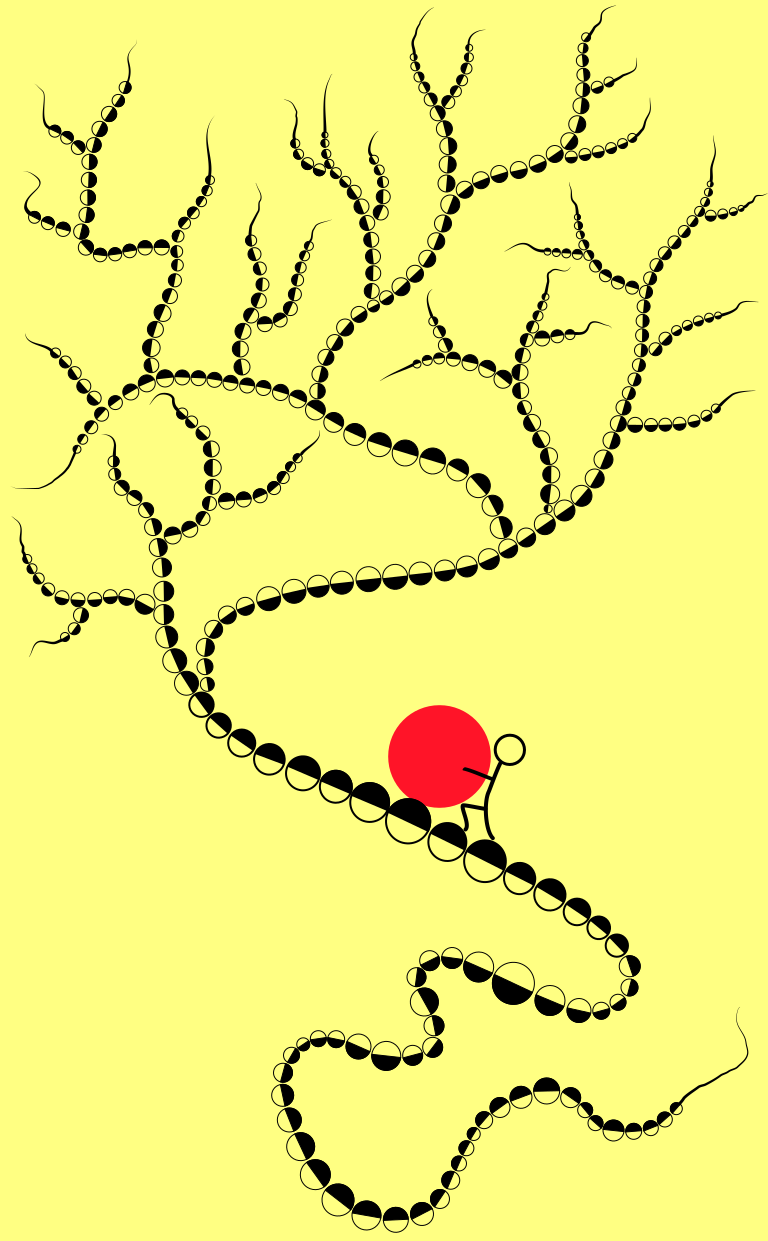
\includegraphics[height=1.5\linewidth]{./cover/syziphus}
\end{center}
\vspace{1em}
\vfill

\begin{center}
	{\Large\bf Miroslav Radojevi\'{c}}
\end{center}

%\end{changemargin}

%\clearpage
%\restoregeometry
%}
% ************************************************************************
% Title Page
% ************************************************************************
\setlength{\parindent}{0pt}
\thispagestyle{empty}
\begin{center}
  \vspace*{5mm}
  {\huge\bf Methods for Automated\\[0.3ex] Neuron Image Analysis\\}
  \vspace{12.85cm}
  {\large\bf Miroslav Radojevi\'{c}}
\end{center}
\setlength{\parindent}{\myindent}



% ************************************************************************
% Colophon
% ************************************************************************

\newpage
\setlength{\parindent}{0pt}
\thispagestyle{empty}

\section*{Colophon}
\addcontentsline{toc}{chapter}{Colophon}

\bigskip
This book was typeset by the author using \LaTeX{}2{\LARGE $_{\varepsilon}$}. The main body of the text was set using a 10-points Computer Modern Roman font. All graphics and figures were created using Inkscape (free and open-source) and Autodesk \textsuperscript{\textregistered}Graphic vector graphics editors and included in the book as Portable Document Format (PDF). % ${}^{\textrm{TM}}\!\!$

\bigskip
Cover design by the author. The graphics on the cover symbolizes the Sisyphus building a neuron tree. We all do Sisyphean work now and then.
\bigskip

\vfill
\includegraphics[height=0.08\textheight]{./logos/emc} % %\rule[0.8mm]{100mm}{0.3mm}

The research described in this thesis was carried out at the Erasmus MC - University Medical Center Rotterdam (Rotterdam, the Netherlands). 
\bigskip

\includegraphics[height=0.08\textheight]{./logos/nwo-nl}

This work was supported by the Netherlands Organization for Scientific Reseach (NWO), grant number 612.001.018 awarded to Erik Meijering.
%Financial support for the publication of this thesis was kindly provided by the Department of Radiology of Erasmus MC -- University Medical Center Rotterdam, and the Erasmus University Rotterdam, the Netherlands.
\bigskip

%\rule[0.8mm]{\textwidth}{0.3mm}
Copyright \copyright\ 2018 by Miroslav Radojevi\'{c}. All rights reserved. No part of this publication may be reproduced or transmitted in any form or by any means, electronic or mechanical, including photocopy, recording, or any information storage and retrieval system, without permission in writing from the author.

\bigskip
ISBN 000-00-0000000-0
\bigskip
Printed by ABC Company
\setlength{\parindent}{\myindent}
% ************************************************************************


% ************************************************************************
%
% Formal page
%
% ************************************************************************

\setlength{\parindent}{0pt}
\thispagestyle{empty}

\begin{center}
  
  \vspace*{5mm}
  {\huge\bf Methods for Automated\\[0.3ex] Neuron Image Analysis\\}

  \vfill
  \vfill
  \vfill

  {\large Methoden voor geautomatiseerde neuronbeeldanalyse\\[1ex]}

%  {\large(met een samenvatting in het Nederlands)}

  \vfill
  \vfill
  \vfill
  \vfill

  {\large\bf Proefschrift}
  {\large 
  \vfill
  \vfill
  
  \normalsize
  
  ter verkrijging van de graad van doctor aan de \\Erasmus Universiteit Rotterdam\\
op gezag van de \\rector magnificus\\
  \vfill
Prof.dr.~A.B.C.~Achtername\\
  \vfill
en volgens besluit van het College voor Promoties. 
  \vfill
De openbare verdediging zal plaatsvinden op \\Dag DD maand YYYY om 0:00 uur
  
  
  \vfill
  \vfill
  
  \large
  door}

  \vfill
  \vfill
  \vfill

  {\large\bf Miroslav Radojevi\'{c}}

  \vfill

  {\large geboren te U\v{z}ice, Servi{\"e}}

  \vfill
  \vfill
\includegraphics[width=0.3\textwidth]{./logos/emc}
\end{center}

% ************************************************************************

\newpage
\thispagestyle{empty}
\label{othersideformal}

\begin{tabular}{@{}ll@{}}
\large\bf{Promotiecommissie} &\\ [8ex]
Promotor:    & {\bf Prof.dr.~W.J.~Niessen}\\[3ex]
Overige leden: & {\bf Prof.dr.ir.~A.B.~Achtername}\\[1ex]
&{\bf Dr.ir.~A.B.~Achtername}\\[1ex]
&{\bf Dr.~A.-B.~Achtername}\\[3ex]
Copromotor: & {\bf Dr.ir.~H.W.~Meijering}\\
\end{tabular}

% \vfill
% %\rule[0.8mm]{100mm}{0.3mm}\hfill\includegraphics[width=0.20\textwidth]{./asci.eps}
% \rule[0.8mm]{\textwidth}{0.3mm}

% %\bigskip

% The research described in this thesis was carried out at the Erasmus MC -- University Medical Center Rotterdam (Rotterdam, the Netherlands). This work was financially supported by the Netherlands Organization for Scientific Research (NWO) through VIDI-grant 639.022.401.

% \bigskip

\setlength{\parindent}{\myindent}

% ************************************************************************


% ***********************************************************************
%
% Preface
% ***********************************************************************
\chpos{14mm}{10mm}
\chapter*{Preface}
\markboth{Preface}{Preface}
\addcontentsline{toc}{chapter}{Preface}

\mysquote{0.8\textwidth}
{The plan is O.K. Only that, for some reason, the events do not stick to it.\newline Plan je O. K. Samo ga se dogadjaji zbog ne\v{c}eg ne dr\v{z}e.}
{Borislav Peki\`{c}, \emph{Rabies} (\oldstylenums{1983})\nocite{}}

%\mysquote{0.8\textwidth}
%{Not everything that can be counted counts, and not everything that counts can be counted.}
%{Albert Einstein (1879-1955)}

%\myquote{0.55\textwidth}{Let no one say that I have said nothing
%	new.\newline The arrangement of the subject is new.}{Blaise Pascal,
%	\emph{Pens\'ees} (\oldstylenums{1670})\nocite{Pascal-1670a}}

%\myquote{0.7\textwidth}{Anyone who does not look back to the beginning
%  throughout a course of action, does not look forward to the end.
%  Hence it necessarily follows that an intention which looks ahead,
%  depends on a recollection which looks back.}{Aurelius Augustinus,
%  \emph{De civitate Dei}, VII.7 (\oldstylenums{417}
%  A.D.)\nocite{Augustin-DeCivitateDei}}
%\noquote

%\noquote

This thesis describes the research carried out as part of my Ph.D. study at the Erasmus University Medical Center Rotterdam. 
\bigskip
\begin{flushright}
  \begin{tabular}{@{}l@{}}
    Miroslav Radojevi\'{c}\\
    Rotterdam, Month 2018.
  \end{tabular}
\end{flushright}
% ************************************************************************

% ************************************************************************
%
% Table of Contents
%
% ************************************************************************

\noquote
\chpos{17mm}{16mm}
\tableofcontents
\cleardoublepage
% ************************************************************************

%%% Local Variables: 
%%% mode: latex
%%% TeX-master: "phdthesis"
%%% End: 


%\glsaddall
%\printglossaries
%\printglossary[style=long]

\printglossary[style=long,type=\acronymtype,title={List of Abbreviations}]

% ************************************************************************
\pagenumbering{arabic}
\setcounter{page}{1}

\setlength{\parindent}{15pt}

\graphicspath{{./chapter1/}}
% ************************************************************************
%
% Introduction
%
% ************************************************************************
\chpos{22mm}{10mm}
\chapter[Introduction]{Introduction}
\markboth{\thechapter\ \ Introduction}{\thechapter\ \ Introduction}
\label{ch1:introduction}

%\mysquote{0.8\textwidth}{Quote text.}{Author (\oldstylenums{1000} - \oldstylenums{1100})}

% ************************************************************************
\section{Neuron cell reconstruction} 
Fascination with the neuron cells dates to the time of the first glance into the sample of the neuronal tissue over a century ago \cite{ramon2008histologia}. Eversince the discovery, and the early hand drawings of the magnified images of the neuronal sample, numerous scientists and researchers with various backgrounds and interests have been trying to gain a better insight into the nervous system and the captivating brain mechanism. Numerous technical obstacles stand out when reaching out to the this vast unknown world, primarily due to the physical inaccessibility. The estimated number of neuron cells in a human brain amounts to 89 billion, number comparable to the total count of stars in the Milky Way galaxy. Each is further connected to 50 thousand other neurons on average which results in a very  computational and storage 

Neuron cells represent a core building block of the brain and the nervous system. 

Captivating mechanism of the brain is an everlasting research topic as the complex functionality of the brain . Discovering how the brain works is central to diverse fields such as physics, mathematics, biology and, recently informatics.

Quantification of the neuronal structure is crucial in neuroscience studies \cite{halavi2012digital}. Neuron reconstruction from microscopic images is identified as one of the major technical challenges in the digital era of neuroscience \cite{peng2015diadem}.

The insights in
\begin{figure}
	\begin{center}
		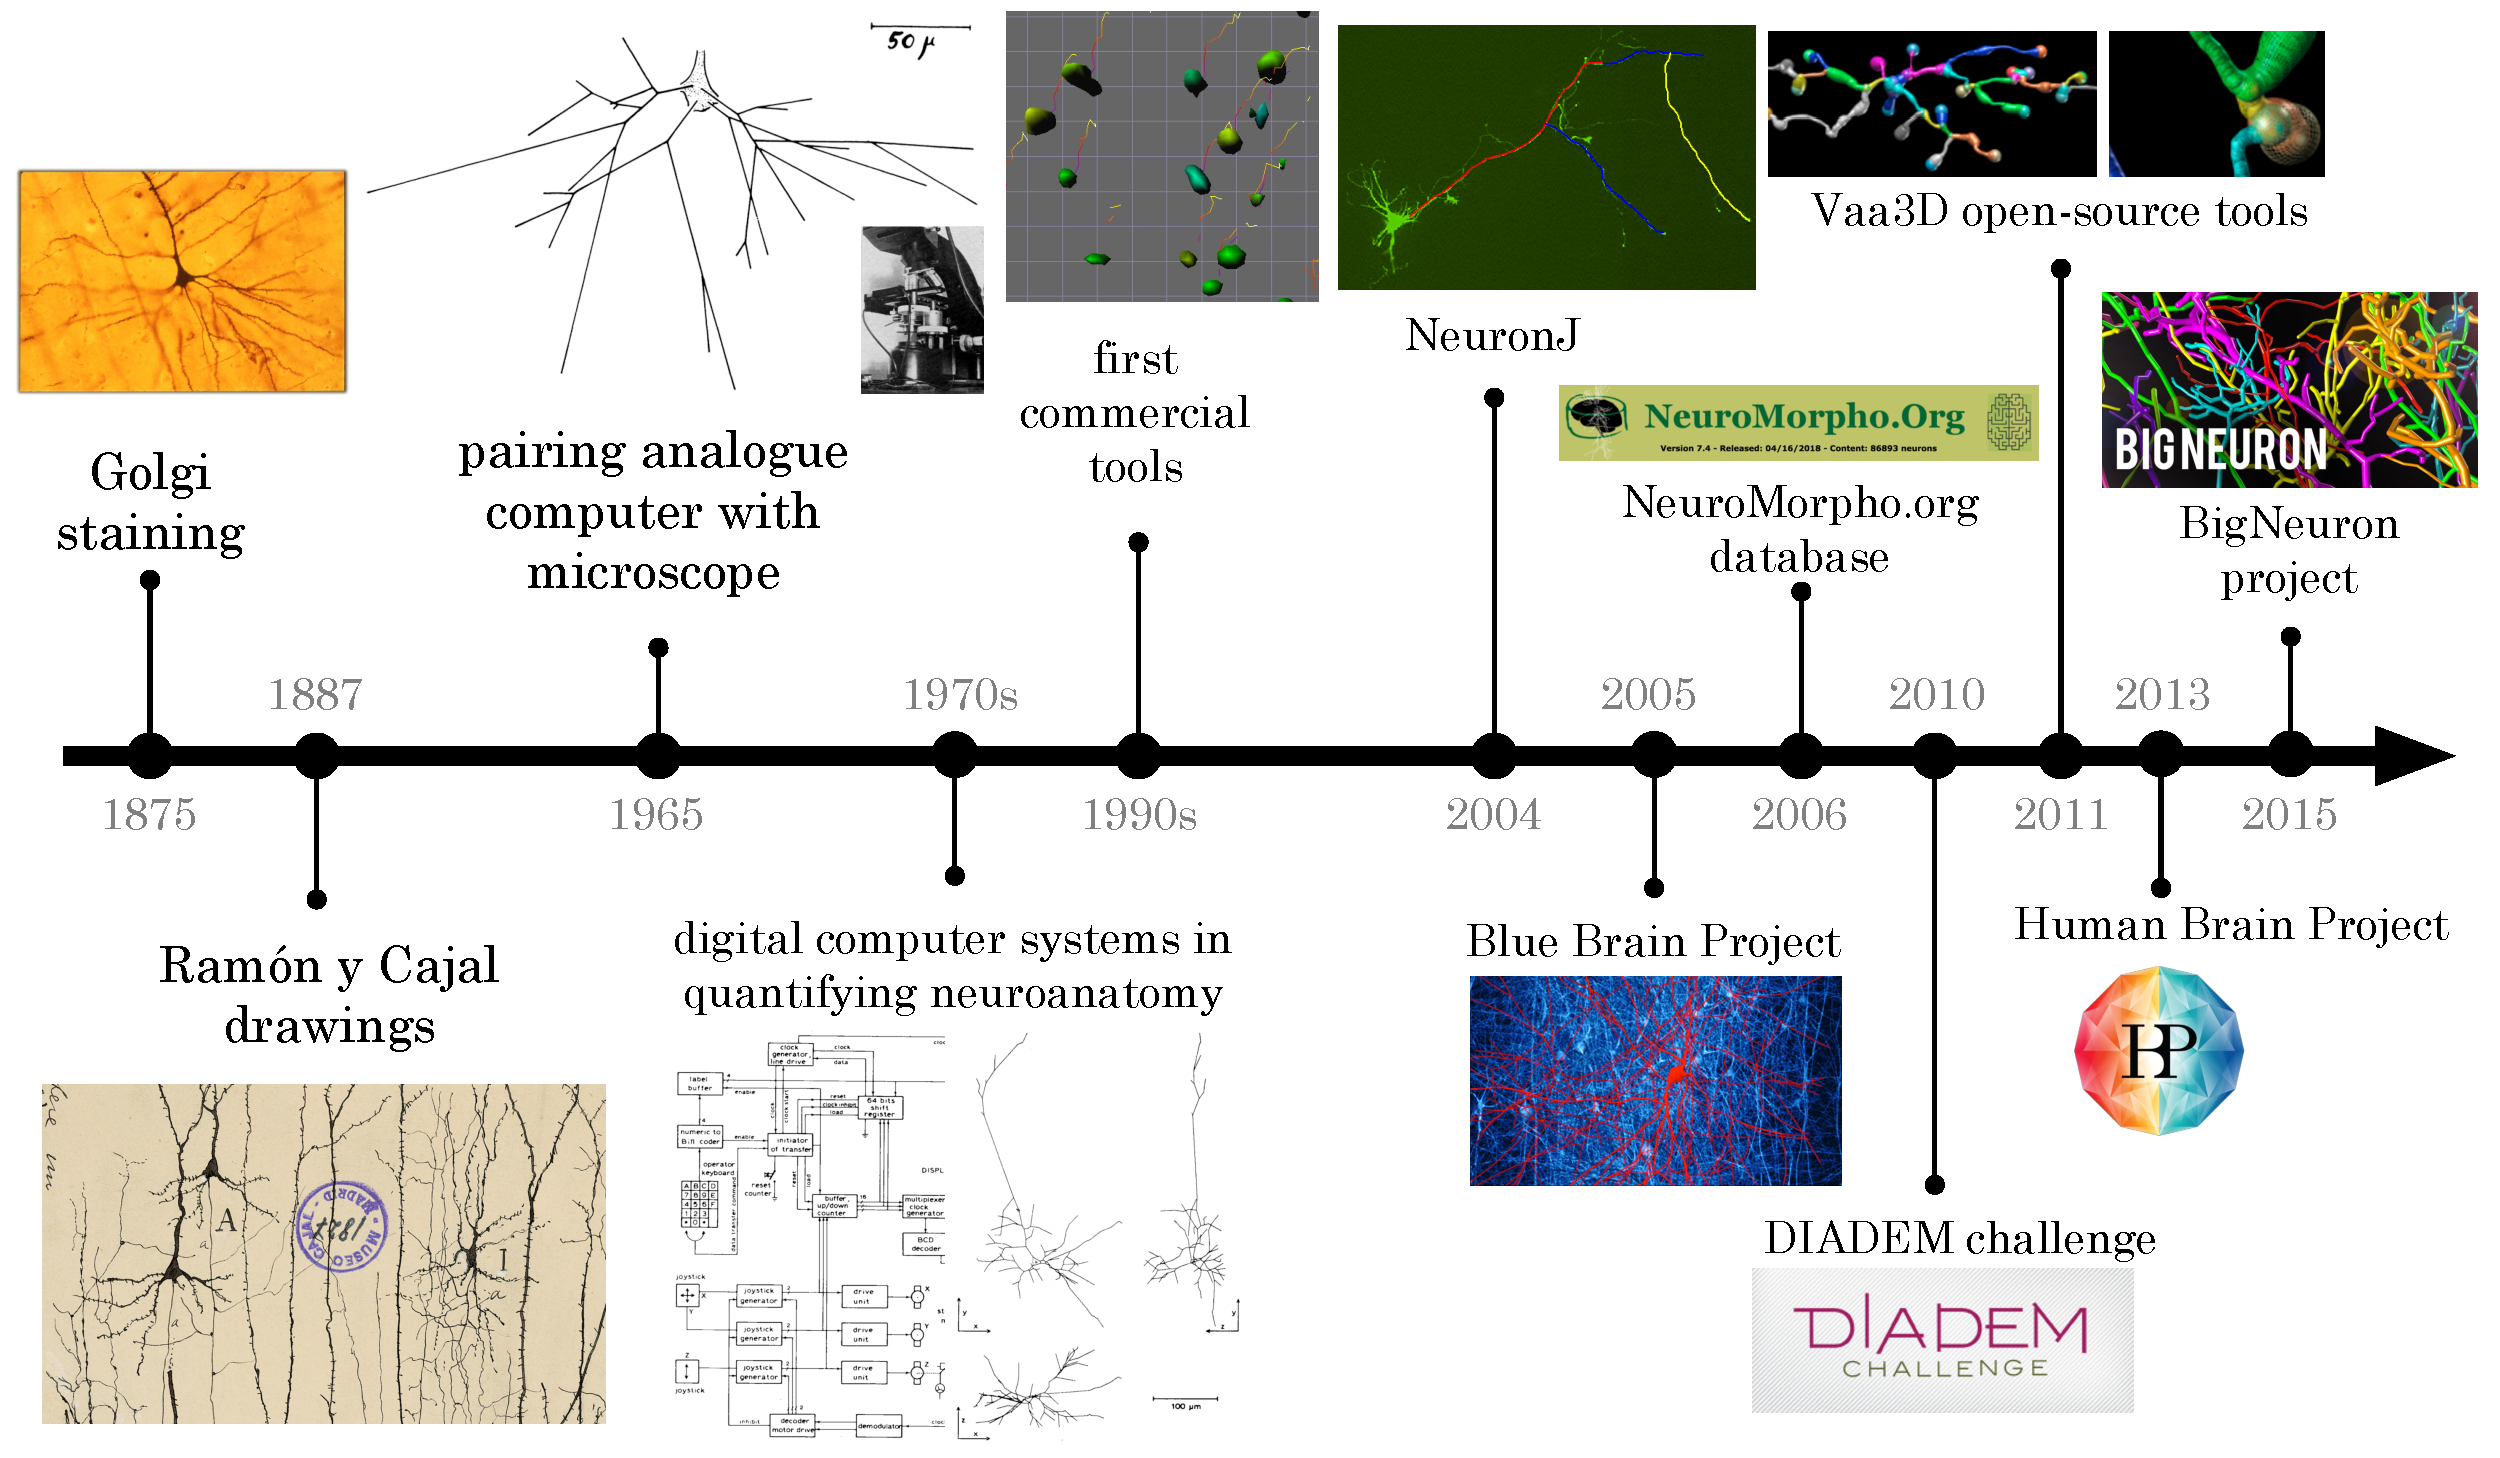
\includegraphics[width=\textwidth]{ch1_fig1}
	\end{center}
	\vspace{-3ex}
	\caption{Neuron reconstruction timeline.}
	\vspace{-1ex}
	\label{ch1__fig1}
\end{figure}

\section{Essential obstacles in neuron reconstruction}

Figure ~\ref{ch1__fig1} represents a neuron reconstruction timeline summary. Several survey publications \cite{meijering2010neuron,donohue2011automated,acciai2016automated}

Microscopic images are capable of .

\section{Tools: notable strategies}
One of the key Java tools is the ImageJ library \cite{abramoff2004image}. 

\begin{figure}
\begin{center}
\includegraphics[width=0.5\textwidth]{ch1_fig2}\\
a) Shortest path tracing \\
\includegraphics[width=0.5\textwidth]{ch1_fig3}\\
b) Minimum spanning tree \\
\includegraphics[width=0.5\textwidth]{ch1_fig4}\\
c) Path-prunning
\end{center}
\vspace{-3ex}
\caption{Examples of key neuron reconstruction strategies: a) Finding optimal path between two fixed points, b) Inferring the  optimal tree structure from the given nodes c) Prunning the overcomplete neuron tree.}
\vspace{-1ex}
\label{ch1__fig2-4}
\end{figure}

Computation methods

\section{Examining the neuronal reconstructions}
SWC format is the .

\begin{figure}
	\begin{center}
		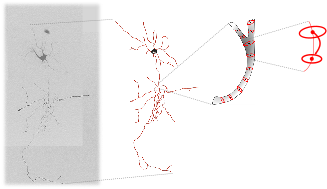
\includegraphics[width=\textwidth]{ch1_fig5}
	\end{center}
	\vspace{-3ex}
	\caption{SWC format of the digital reconstruction, Stockley, Wheal and Cole \cite{stockley1993system}. Visualization using Vaa3D \cite{peng2010automatic}}
	\vspace{-1ex}
	\label{ch1__fig5}
\end{figure}

Distances between neurons can be based on the overlap and the inter-node metric distances.

\section{Thesis outline}
In this thesis.


\graphicspath{{./chapter2/}}
% ************************************************************************
% 
%
% ************************************************************************

\myquote{0.55\textwidth}{Let no one say that I have said nothing
  new.\newline The arrangement of the subject is new.}{Blaise Pascal,
  \emph{Pens\'ees} (\oldstylenums{1670})\nocite{Pascal-1670a}}


\noquote

\chpos{15mm}{8mm}
\chapter[Quantitative Comparison of Spot Detection Methods in\\
 Fluorescence Microscopy]{Quantitative Comparison \\of Spot Detection Methods \\in Fluorescence Microscopy}
\chaptermark{Quantitative Comparison of Spot Detection Methods}
\label{ch2__chaprter2}

\mysquote{\textwidth}
{Not everything that can be counted counts, and not everything that
  counts can be counted.}
{Albert Einstein (1879-1955)}



% ************************************************************************
% ************************************************************************
\myabstract{
Quantitative analysis of biological image data generally involves the detection of many subresolution spots.
Especially in live cell imaging, for which fluorescence microscopy is often used, the signal-to-noise ratio (SNR) can be extremely low,
making automated spot detection a very challenging task. In the past, many methods have been proposed to perform this task,
but a thorough quantitative evaluation and comparison of these methods is lacking in the literature.
In this chapter, we evaluate the performance of the most frequently used detection methods for this purpose.
These include six unsupervised and two supervised methods.
We perform experiments on synthetic images of three different types,
for which the ground truth was available,
as well as on real image data sets acquired for two different biological studies,
for which we obtained expert manual annotations to compare with.
The results from both types of experiments suggest that for very low SNRs ($\approx$2),
the supervised (machine learning) methods perform best overall.
Of the unsupervised methods, the detector based on the so-called
$h$-dome transform from mathematical morphology 
performs comparably, and has the advantage that it does not require a cumbersome learning stage.
At high SNRs ($>$5), the difference in performance of all considered detectors becomes negligible.}

\smallskip

% ************************************************************************
% ************************************************************************

\begin{publish}
Based upon: M. Radojevi\'{c}, I. Smal, E. Meijering, ``Fuzzy logic based'', \textit{in press}.   
\end{publish}

\section{Introduction}
\label{ch2__sec:intro}
\dropping{3}{T}he very first stage in the analysis of biological image data generally deals with the detection of objects of interest.

\graphicspath{{./chapter3/}}
% ************************************************************************
%
% Automated neuron tracing using probability hypothesis density filtering
%
% ************************************************************************
\chpos{15mm}{8mm}
\chapter[Automated neuron tracing using probability hypothesis density filtering]{Automated neuron tracing using probability hypothesis density filtering}
\chaptermark{Automated neuron tracing using probability hypothesis density filtering}
\label{ch3:phd}

\myabstract{\lettrine{T}{he} functionality of neurons and their role in neuronal networks is tightly connected to the cell morphology. A fundamental problem in many neurobiological studies aiming to unravel this connection is the digital reconstruction of neuronal cell morphology from microscopic image data. Many methods have been developed for this, but they are far from perfect, and better methods are needed. Here we present a new method for tracing neuron centerlines needed for full reconstruction. The method uses a fundamentally different approach than previous methods by considering neuron tracing as a Bayesian multi-object tracking problem. The problem is solved using probability hypothesis density filtering. Results of experiments on 2D and 3D fluorescence microscopy image datasets of real neurons indicate the proposed method performs comparably or even better than the state of the art.}

%\smallskip
%\bigskip
\vfill
\vspace{23em}
% ************************************************************************
\begin{publish}
	Based upon: M. Radojevi\'{c}, E. Meijering, ``Automated neuron tracing using probability hypothesis density filtering'', \textit{Bioinformatics}, vol. 33, no. 7, pp.1073-1080, 2017.   
\end{publish}

\section{Introduction}
\label{ch3_sec_intro}

\graphicspath{{./chapter4/}}
% ************************************************************************
%
% Automated neuron tracing using probability hypothesis density filtering
%
% ************************************************************************
\chpos{15mm}{8mm}
\chapter[Automated neuron tracing using probability hypothesis density filtering]{Automated neuron tracing using probability hypothesis density filtering}
\chaptermark{Automated neuron tracing using probability hypothesis density filtering}
\label{ch3:phd}

\myabstract{\lettrine{T}{he} functionality of neurons and their role in neuronal networks is tightly connected to the cell morphology. A fundamental problem in many neurobiological studies aiming to unravel this connection is the digital reconstruction of neuronal cell morphology from microscopic image data. Many methods have been developed for this, but they are far from perfect, and better methods are needed. Here we present a new method for tracing neuron centerlines needed for full reconstruction. The method uses a fundamentally different approach than previous methods by considering neuron tracing as a Bayesian multi-object tracking problem. The problem is solved using probability hypothesis density filtering. Results of experiments on 2D and 3D fluorescence microscopy image datasets of real neurons indicate the proposed method performs comparably or even better than the state of the art.}

\graphicspath{{./chapter5/}}
% ************************************************************************
%
% Automated neuron detection in high-content fluorescence microscopy images
% using machine learning 
%
% ************************************************************************
%Automated neuron detection in high-content fluorescence microscopy images using machine learning
\chpos{15mm}{8mm}
\chapter[Automated neuron detection in high-content fluorescence microscopy images using machine learning]{Automated neuron detection in high-content fluorescence microscopy images using machine learning}
\chaptermark{Automated neuron detection in high-content images using machine learning}
\label{ch5:ndetchml}
% abstract
{\small \lettrine{T}{he} study of neuronal morphology in relation to function, and the development of effective medicines to positively impact this relationship in patients suffering from neurodegenerative diseases, increasingly involves image-based high-content screening and analysis. The first critical step toward fully automated high-content image analyses in such studies is to detect all neuronal cells and distinguish them from possible non-neuronal cells or artifacts in the images. Here we investigate the performance of well-established machine learning techniques for this purpose. These include support vector machines, random forests, k-nearest neighbors, and generalized linear model classifiers, operating on an extensive set of image features extracted using the compound hierarchy of algorithms representing morphology, and the scale-invariant feature transform. We present experiments on a dataset of rat hippocampal neurons from our own studies to find the most suitable classifier(s) and subset(s) of features in the common practical setting where there is very limited annotated data for training. The results indicate that a random forests classifier using the right feature subset ranks best for the considered task, although its performance is not statistically significantly better than some support vector machine based classification models.\par}
\vspace*{12em}
% ************************************************************************
\begin{publish}
	Based upon: G. Mata, M. Radojevi\'{c}, C. Fernandez-Lozano, I. Smal, M. Morales, E. Meijering, J. Rubio, ``Automated neuron detection in high-content fluorescence microscopy images using machine learning'', \textit{Neuroinformatics}, \textit{in review}
\end{publish}%vol. 0, no. 0, pp.0-0, 2018.

\section{Introduction}
\label{sec:intro}
Neurons are special cells in the sense that they codify and transmit information in the form of action potentials. Networks consisting of many billions of neurons, such as in the brains of higher organisms, are extraordinarily complex and perform many different functions. Since the pioneering work of \cite{ramon2008histologia} it is well known that the morphology of neurons vary widely in different parts of the brain and that neuronal morphology and function are intricately linked. Moreover, in healthy conditions, neuronal (sub)networks within the brain are dynamic and continuously readjust their connections during the lifetime of an organism in response to external stimuli, in order to refine existing functions or learn new ones \cite{ascolitrees}. Conversely, in pathological conditions, disease processes destructively alter neuronal morphology and cause progressive loss of function, such as in Alzheimer's and Parkinson's disease, but also in aging \cite{van2001need}. Thus the study of neuronal cell morphology in relation to function, in health and disease, is of high importance for developing suitable drugs and therapies \cite{meijering2010neuron}.

A convenient tool to visualize large numbers of cultured cells for phenotypic profiling and analysis in drug discovery is high-content fluorescence microscopy imaging \cite{xia2012concise, Antony-2013, Singh-2014, Bougen-Zhukov-2017}. By automated acquisition it produces very large amounts of image data, which cannot be analyzed manually but require automated high-content analysis (HCA) in order to take full advantage of all captured information. HCA is also used increasingly in neuroscience research \cite{D08, ARB09, Jain-2012} and various image processing pipelines have been developed for quantitative analysis of neuronal cells in high-content images \cite{Vallotton-2007, Zhang-2007, Wu-2010, Dehmelt-2011, RN12, Charoenkwan-2013, Smafield-2015}. However, especially in screening applications, where the image quality is often relatively low and may vary widely between experiments, the challenge remains to develop more accurate and more robust image analysis methods \cite{Sommer-2013, Kraus-2016, Meijering-2016}.
% ************************************************************************
%
% Bibliography
%
% ************************************************************************
\cleardoublepage
\addcontentsline{toc}{chapter}{Bibliography}
\chapter*{Bibliography}
\markboth{Bibliography}{Bibliography}
\chpos{25mm}{8mm}

 \mysquote{0.8\textwidth}
 {Simplicity is prerequisite for reliability.\vspace{4mm}}
 {Edsger Dijkstra, \oldstylenums{1930} - \oldstylenums{2002}}

{\footnotesize
\bibliography{./literature}
}

% ************************************************************************
%
% Samenvatting
%
% ************************************************************************
\noquote
\selectlanguage{dutch}

\chpos{22mm}{12mm}
\chapter*{Samenvatting}
\markboth{Samenvatting}{Samenvatting}
\addcontentsline{toc}{chapter}{Samenvatting}

\lettrine{N}{euronen} behoren tot de belangrijkste elementen van het zenuwstelsel. Fascinatie voor deze cellen gaat minstens terug tot het baanbrekende werk van Ram\'{o}n y Cajal, nu meer dan een eeuw geleden. Gewapend met een microscoop en gebruikmakend van zilverkleuring, niet lang daarvoor ontdekt door Golgi, bestudeerde hij hersenweefsels uit een groot aantal gebieden van de hersenen. Zijn bevindingen leidden tot het opstellen van de neuronentheorie, die stelt dat het zenuwstelsel, net als alle andere organen in het lichaam, is opgebouwd uit afzonderlijke cellen. Golgi en Ram\'{o}n y Cajal deelden in 1906 de Nobelprijs voor Geneeskunde. Daarop volgend grondig onderzoek naar neuronen onthulde dat deze cellen de bijzondere eigenschap hebben dat ze signalen kunnen ontvangen en doorgeven. Daarmee regelen ze een groot aantal lichaamsfuncties. Ook werd duidelijk dat neuronen in de verschillende delen van de hersenen verschillende functies hebben. Afhankelijk van hun specifieke rol in het zenuwstelsel kunnen neuronen nogal variëren in hun morfologische eigenschappen.

Morfologische analyse van de verschillende soorten neuronen is daarom vaak een belangrijk onderdeel in het onderzoek naar hun functie. Neuronen kunnen tegenwoordig in groot detail en digitaal worden afgebeeld door middel van moderne lichtmicroscopen. Maar om de eigenschappen van een gegeven neuron daadwerkelijk te kunnen kwantificeren is een explicietere representatie van zijn morfologie nodig dan een microscoopbeeld. Het afleiden van een grafische representatie van een neuron uit zijn microscoopbeeld, in de vorm van een boomstructuur bestaande uit knooppunten en vertakkingen, wordt doorgaans aangeduid als digitale reconstructie, en is het hoofdthema van dit proefschrift. Veel neurowetenschappelijke studies zijn afhankelijk van een nauwkeurige beschrijving van de morfologie van neuronen in de vorm van digitale reconstructies. Daarmee is digitale reconstructie een belangrijk technisch probleem in neurowetenschappelijk onderzoek.

Dit proefschrift presenteert nieuwe computationele methoden voor de automatische analyse van neuronen. De hoofdproblemen waarvoor oplossingen worden gepresenteerd zijn de detectie en de reconstructie van neuronen in digitale fluorescentiemicroscopiebeelden. Een van de belangrijkste vernieuwingen die worden voorgesteld ten opzichte van bestaande reconstructiemethoden is het gebruik van probabilistische filtertechnieken. Na een algemene inleiding in het eerste hoofdstuk, beschrijven de daarop volgende hoofdstukken originele oplossingen voor de automatische detectie van knooppunten en eindpunten van neuronen in hun afbeeldingen, het traceren van alle vertakkingen van de neuronen in de beelden, en het vinden van neuronen in lageresolutiebeelden uit screeningstudies. De rest van deze samenvatting geeft kort de inhoud van de hoofdstukken weer.

Het tweede hoofdstuk presenteert een nieuwe methode voor de automatische detectie van die punten in beelden van neuronen die van cruciaal belang zijn voor de correcte topologische representatie van de neuronen. Het gaat hierbij vooral om de knooppunten en de eindpunten van alle vertakkingen. Een knooppunt is een punt waar drie segmenten van de boomstructuur bij elkaar komen, en een eindpunt is een punt waar een vertakking van de boomstructuur eindigt. De voorgestelde detectiemethode maakt gebruik van richtingsfilters, waarmee in elk punt van een beeld wordt bepaald in hoeverre en in welke richting(en) er lijnachtige structuren door het punt lopen. De gevonden informatie hierover wordt uitgedrukt in taalkundige termen die vervolgens verwerkt worden door middel van zogeheten vage logica. Daarmee wordt elk punt met behulp van een stelsel van regels geclassificeerd als zijnde irrelevant of een specifiek type cruciaal punt uit de boomstructuur van het neuron. Voor dit doel wordt een nieuw stelsel van regels en klassen voorgesteld. De kracht van de gekozen aanpak is dat voor elk punt berekend wordt in welke mate het behoort tot elk van de beschouwde klassen. Daardoor wordt rekening gehouden met de onzekerheid in de beeldinformatie en het filterproces.

In het derde hoofdstuk wordt het theorema van Bayes benut om te komen tot een nieuwe automatische methode voor het traceren van de middellijn van neuronale vertakkingen in microscoopbeelden. In tegenstelling tot bestaande methoden is de voorgestelde methode probabilistisch van aard en in staat om tegelijkertijd een onbeperkt aantal vertakkingen te traceren. Voor de implementatie van de methode wordt gebruik gemaakt van sequentiële Monte Carlo filtering. Een dergelijke aanpak wordt ook wel gebruikt in andere toepassingen, voor het volgen van bewegende objecten over de tijd in filmopnames. In dit hoofdstuk wordt het idee echter aangewend voor het volgen van objecten in de ruimte in statische opnames. Om dit mogelijk te maken worden nieuwe wiskundige modellen voorgesteld voor het filterproces, waarin bestaande kennis is opgenomen over de vorm van neuronale vertakkingen en de manier waarop ze worden afgebeeld door een microscoop. De probabilistische aard van de methode maakt dat herhaalde toepassing op hetzelfde beeld net iets andere resultaten oplevert. Op deze manier kan meer statistisch bewijsmateriaal worden vergaard over de vorm van de vertakkingen dan dat deterministische methoden kunnen leveren. De gepresenteerde experimentele resultaten bevestigen inderdaad dat de methode nauwkeuriger is.

Het vierde hoofdstuk tilt het idee van probabilistische tracing nog een stap verder en presenteert een nieuwe methode voor automatische volledige reconstructie van neuronen uit microscoopbeelden. Deze methode vindt niet alleen de middellijn van individuele vertakkingen, maar maakt ook een schatting van de lokale diameter op elk punt van de vertakkingen, en voegt alle gevonden segmenten samen tot een datastructuur die de berekening van allerlei morfologische eigenschappen mogelijk maakt. De methode begint met het identificeren van die gebieden in een beeld die hoogstwaarschijnlijk neuronale vertakkingen bevatten. Voor dit doel wordt een bestaande buisfiltermethode gebruikt. Uit de gevonden gebieden worden vervolgens startpunten geselecteerd voor het traceren van de vertakkingen. Net als in het voorgaande hoofdstuk wordt hiervoor een probabilistische aanpak gebruikt op basis van sequentiële Monte Carlo filtering. Ook hier levert herhaalde toepassing meer informatie over de vertakkingen en leidt tot betere resultaten. Tevens zij opgemerkt dat de herhalingen onafhankelijk zijn van elkaar en zich dus uitstekend lenen voor parallelle implementatie. Om een volledige reconstructie te verkrijgen worden de resultaten van de verschillende herhalingen verfijnd en samengevoegd. Hiervoor worden nieuwe iteratieve algoritmes voorgesteld. Een eerste versie van de methode is opgenomen in een internationale vergelijkingsstudie genaamd BigNeuron, waar het als een van de betere methoden uit de bus kwam. In dit hoofdstuk wordt een sterk verbeterde versie gepresenteerd.

Tenslotte wordt in het vijfde hoofdstuk een haalbaarheidsstudie gepresenteerd van het detecteren van gebieden in lageresolutiebeelden van celculturen die neuronen bevatten. Deze taak is doorgaans de eerste stap in screeningstudies naar de aantasting van neuronen door neurodegeneratieve ziektes en het effect van medicijnen. De gevonden gebieden worden vervolgens afgebeeld op hoge resolutie, waarna de neuronen kunnen worden gereconstrueerd met behulp van de in de vorige hoofdstukken beschreven methoden. De detectie in de lageresolutiebeelden wordt bemoeilijkt door de afwezigheid van details, het feit dat de neuronen vaak niet volledig zijn afgebeeld, de aanwezigheid van vergelijkbare cellen zoals astrocyten, en beeldvormingsartefacten zoals (veel) ruis. Daarom is in deze studie gekozen voor het gebruik van zelflerende methoden op basis van beeldkenmerken berekend door een zeer groot aantal bestaande filtertechnieken. In de gepresenteerde experimenten worden de prestaties van vier soorten traditionele zelflerende methoden vergeleken. Ook wordt een proefexperiment beschreven met een tegenwoordig zeer populaire aanpak op basis van kunstmatige, dieplerende neurale netwerken. De conclusie is echter dat op deze beperkte data de traditionele methoden beter presteren.

% ************************************************************************
\selectlanguage{english}
% ************************************************************************


% ************************************************************************
%
% Curriculum Vitae
%
% ************************************************************************

\noquote
\orgchpos
\chapter*{PhD Portfolio}
\markboth{PhD Portfolio}{PhD Portfolio}
\addcontentsline{toc}{chapter}{PhD Portfolio}

% ************************************************************************
\noindent

\subsection*{Research Skills:}
\vspace{1ex}
\begin{itemize}
	\item B.Sc. degree in Electrical Engineering, Faculty of Electrical Engineering - University of Belgrade, Serbia, 2008
	\item M.Sc. degree in Computer Vision and Robotics, Heriot-Watt University, Scotland, 2011
	\item Professional Doctorate in Engineering (PDEng) degree, Technical
University of Eindhoven, the Netherlands, 2005
\end{itemize}

\subsection*{In-Depth Courses:}
\vspace{1ex}
\begin{itemize}
\item Knowledge driven Image Segmentation, ASCI, 2005
\item Measuring Features, ASCI, 2006
\item Front-End Vision and Multiscale Image Analysis, ASCI, 2007
\item BioInformatics, ASCI, 2007
\end{itemize}

\subsection*{International Conference Presentations:}
\vspace{1ex}
\begin{itemize}
\item IEEE International Symposium on Biomedical Imaging: From Nano to Macro --- ISBI~2006,
Arlington, VA, USA, April 6--9, 2006
\item IEEE Nonlinear Statistical Signal Processing Workshop: Classical,
    Unscented and Particle Filtering Methods --- NSSPW~2006, Cambridge, UK, September 13-15, 2006
\item IEEE International Symposium on Biomedical Imaging: From Nano to
  Macro --- ISBI~2007, Arlington, VA, USA, April, 12--15, 2007
\item Information Processing in Medical Imaging --- IPMI~2007, Kerkrade, the Netherlands, July 2-6,
2007
\item IEEE International Symposium on Biomedical Imaging: From Nano to
  Macro --- ISBI~2008, Paris, France, May 14--17, 2008
\end{itemize}

\subsection*{Invited Lectures and Seminars:}
\vspace{1ex}
\begin{itemize}
\item Promovendidagen 2006, Maastricht, January 26-27, 2006
\item Medical Imaging Symposium for PhD-Students, University Medical Center Utrecht, January 11, 2007
\end{itemize}

\subsection*{Travel Grants:}
\vspace{1ex}
\begin{itemize}
\item Student travel grant, IEEE International Symposium on Biomedical Imaging: From Nano to
  Macro --- ISBI~2007, Arlington, VA, USA, April, 12--15, 2007
\end{itemize}

\subsection*{Other:}
\vspace{1ex}
\begin{itemize}
\item Referee activities for various international scientific journals
 (IEEE Transactions on Medical Imaging, IEEE
  Transactions on Image Processing, IEEE Transactions on Biomedical
  Engineering, Image and Vision Computing, Sensors) and international
  conferences (IEEE International Conference on Image
    Processing (ICIP) and International Conference on Medical Image Computing and Computer
    Assisted Intervention (MICCAI))
\end{itemize}

% ************************************************************************
%
% Publications
%
% ************************************************************************

\noquote
\orgchpos
\chapter*{Publications}
\markboth{Publications}{Publications}
\addcontentsline{toc}{chapter}{Publications}
\label{publications}

\small
\normalsize

\subsection*{Publications in International Journals:}
\vspace{1ex}
\begin{itemize}
	\item \textbf{M.~Radojevi\'{c}}, I.~Smal, E.~Meijering, ``Fuzzy-Logic Based Detection and Characterization of Junctions and Terminations in Fluorescence Microscopy Images of Neurons'', \emph{Neuroinformatics}, vol.~11, no.~11, pp.~1-11, 2015
	
	\item \textbf{M.~Radojevi\'{c}}, E.~Meijering, ``Automated Neuron Tracing using Probability Hypothesis Density Filtering'', \emph{Bioinformatics}, vol.~33, no.~7, pp.~1073-1080, 2017
	
	\item V.~Ulman, M.~Ma\v{s}ka, K.~E.~G.~Magnusson, O.~Ronneberger, C.~Haubold, N.~Harder, P.~Matula, P.~Matula, D.~Svoboda, \textbf{M.~Radojevi\'{c}}, I.~Smal, K.~Rohr, J.~Jald\'{e}n, H.~M.~Blau, O.~Dzyubachyk, B.~Lelieveldt, P.~Xiao, Y.~Li, S.~Y.~Cho, A.~C.~Dufour,	J.~C.~Olivo-Marin, C.~C.~Reyes-Aldasoro, J.~A.~Solis-Lemus, R.~Bensch, T.~Brox, J.~Stegmaier, R.~Mikut, S.~Wolf,	F.~A.~Hamprecht, T.~Esteves, P.~Quelhas, \"{O}.~Demirel, L.~Malmstr\"{o}m, F.~Jug, P.~Tomancak, E.~Meijering, A.~Mu\~{n}oz-Barrutia, M.~Kozubek, C.~Ortiz-de-Solorzano ``An Objective Comparison of Cell-tracking Algorithms'', \emph{Nature Methods}, vol.~14, no.~12, pp.~1141-1152, 2017
	
	\item \textbf{M.~Radojevi\'{c}}, E.~Meijering, ``Automated Neuron Reconstruction from 3D Fluorescence Microscopy Images using Sequential Monte Carlo Estimation'', \emph{Neuroinformatics}, \emph{in review}%vol.~0, no.~0, pp.~0-0, 2018
	
	\item G.~Mata, \textbf{M.~Radojevi\'{c}}, C.~Fernandez-Lozano, I.~Smal, N.~Werij, M.~Morales, E.~Meijering, J.~Rubio, ``Automated Neuron Detection in High-content Fluorescence Microscopy Images using Machine Learning'', \emph{Neuroinformatics}, \emph{in review}%vol.~0, no.~0, pp.~0-0, 2018
\end{itemize}

\subsection*{Publications in International Conference Proceedings:}
\vspace{1ex}
\begin{itemize}
	\item L.~\v{S}ajn, \textbf{M.~Radojevi\'{c}}, T.~Dobravec, ``3D Volume Localization using Miniatures'', in \emph{IEEE International Convention on Information and Communication Technology, Electronics and Microelectronics --- MIPRO 2014} (37th international conference, held in Opatija, Croatia, May 26--30, 2014), IEEE, Piscataway, NJ, pp.~411--416, 2014

	\item \textbf{M.~Radojevi\'{c}}, I.~Smal, W.~Niessen, E.~Meijering, ``Fuzzy Logic Based Detection of Neuron Bifurcations in Microscopy Images'', in \emph{IEEE International Symposium on Biomedical Imaging: From Nano to Macro --- ISBI 2014} (11th international conference, held in Beijing, China, April 29--May 2, 2014), G. Wang and B. He (eds.), IEEE, Piscataway, NJ, pp.~1307--1310, 2014

	\item \textbf{M.~Radojevi\'{c}}, I.~Smal, E.~Meijering, ``Automated Neuron Morphology Reconstruction using Fuzzy-logic Detection and Bayesian Tracing Algorithms'', in \emph{IEEE International Symposium on Biomedical Imaging: From Nano to Macro --- ISBI 2015} (12th international conference, held in New York, NY, USA, April 16--19, 2015), E. Angelini and J. Kova\v{c}evi\'{c} (eds.), IEEE, Piscataway, NJ, pp.~885--888, 2015

	\item G.~Mata, \textbf{M.~Radojevi\'{c}}, I.~Smal, M.~Morales, E.~Meijering, J.~Rubio, ``Automatic Detection of Neurons in High-content Microscope Images using Machine Learning Approaches'', in \emph{IEEE International Symposium on Biomedical Imaging: From Nano to Macro --- ISBI 2016} (13th international conference, held in Prague, Czech Republic, April 13--16, 2016), J. Kybic and M. \v{S}onka (eds.), IEEE, Piscataway, NJ, pp.~330--333, 2016

	\item \textbf{M.~Radojevi\'{c}}, E.~Meijering, ``Neuron Reconstruction from Fluorescence Microscopy Images using Sequential Monte Carlo Estimation'', in \emph{IEEE International Symposium on Biomedical Imaging: From Nano to Macro --- ISBI 2017} (14th international conference, held in Melbourne, VIC, Australia, April 18--21, 2017), G. Egan and O. Salvado (eds.), IEEE, Piscataway, NJ, pp.~36--39, 2017 

\end{itemize}

\normalsize

% ************************************************************************
%
% Curriculum Vitae
%
% ************************************************************************

\noquote
\orgchpos
\chapter*{Curriculum Vitae}
\markboth{Curriculum Vitae}{Curriculum Vitae}
\addcontentsline{toc}{chapter}{Curriculum Vitae}

% ************************************************************************
\noindent
%Miroslav Radojevi\'{c} was born in U\v{z}ice, Serbia, on January 7, 1984. He received a B.Sc. in electrical engineering (control systems) from the Faculty of Electrical Engineering, University of Belgrade, Serbia. Subsequently, he completed M.Sc. degree in Computer Vision and Robotics from the ViBot Erasmus Mundus programme hosted in cooperation by Heriot-Watt University (Scotland), Universit\`{e} de Bourgogne (France) and Universit\"{a}t de Girona (Spain) in 2011. 
%%From 2012 to 2016, he was a conducted the  Scientist at the Electrical Engineering department of the same university. During that period he carried out research in the field of nonlinear and chaotic dynamical systems. 
%
%\bigskip
%\noindent
%During , he was a Research Assistant (postmaster program ``Mathematics for Industry'') at the department of Mathematics and Computer Science of Technical University of Eindhoven, the Netherlands. In 2005 he graduated on the project ``Design and implementation of a six camera scanning unit'' and was awarded a Professional Doctorate in Engineering degree (PDEng). 
%
%\bigskip
%\noindent
%From Dec. 2012 to Feb. 2016 he was a Ph.D. student at the Departments of Medical Informatics and Radiology of the Erasmus University Rotterdam, the Netherlands. His research topic was tracking and motion analysis in cellular and molecular bioimaging. The project was carried out in collaboration with the Department of Cell Biology and Department of Pathology at Erasmus MC Rotterdam. The results are described in this thesis.
%
%\bigskip
%\noindent
%Since 2017. he has been working as software engineer with the research and development department of Becton, Dickinson and Company (BD) focused on the development of medical devices.

% ************************************************************************
\end{document}
% ************************************************************************
